\documentclass[10pt,twocolumn,letterpaper]{article}

\usepackage{cvpr}
\usepackage{times}
\usepackage{epsfig}
\usepackage{graphicx}
\usepackage{amsmath}
\usepackage{amssymb}
\usepackage{wrapfig}

\usepackage{algorithm,algpseudocode}

\DeclareMathOperator*{\argmin}{arg\,min}
\newcommand{\cs}[1]{\texttt{\symbol{`\\}#1}}

\usepackage[breaklinks=true,bookmarks=false]{hyperref}


\cvprfinalcopy % *** Uncomment this line for the final submission
\def\cvprPaperID{****} % *** Enter the CVPR Paper ID here
\def\httilde{\mbox{\tt\raisebox{-.5ex}{\symbol{126}}}}

\graphicspath{{Figures/}{../Figures/}}

\setcounter{page}{1}
\begin{document}

%%%%%%%%% TITLE
\title{CME 338 Final Paper: Hessian-free optimization for training convolutional neural networks in Tensorflow}

\author{Adele Kuzmiakova\\
Stanford University\\
{\tt\small adele.kuzmiakova@stanford.edu}
}
\maketitle

ABSTRACT

Second-order methods for deep learning optimization enjoy several advantages over first-order methods, including no need for extensive hyperparameter tuning, faster convergence rates, and better scaling to large mini batch sizes. Despite these strengths, second-order algorithms are rarely applied in practice due to their high computational cost. We test several Hessian free variants, which aim to approximate the local curvature of the loss function, allowing us to compute more efficient updates. We also implement and test several preconditioners in order to reduce the number of conjugate gradient (CG) iterations. Experiments with these Hessian free variants in the context of convolutional neural networks with multiple convolutional layers show better convergence and generalization than a stochastic gradient descent (SGD) method. Moreover, the performance of the Hessian free methods is on par with the Adam optimizer. One of the barriers for a large-scale adoption of the Hessian free optimizer in Tensorflow is long training time, which could possibly be taken care of by a block-diagonal approximation of the curvature matrix.

\section{Introduction}
\label{sec:introduction}

Optimization algorithms used in deep learning play an important role in the training of the neural networks; they are designed to minimize an objective function consisting of the model's internal learnable parameters, such as weights and bias terms. First order methods, which solely rely on gradient information of the objective function, are simple to design and implement. Traditionally, SGD methods have been one of the most  extensively employed first-order methods throughout the last several decades ~\cite{LeCun98, Zinkevich10}. The central idea is to use gradient to form a linear approximation and take the step towards the minima of that approximation. Key advantages of SGDs are that they are simple to implement and are fast in training neural networks with many training examples ~\cite{Bottou10}. Yet, despite their ease of implementation, SGDs come with several disadvantages. One prominent drawback of SGDs is that they require manual fine-tuning of hyperparameters ~\cite{Berahas17}, such as learning rate and convergence criterion, which are often problem-specific and not known apriori. A standard strategy in this case is to run the learning algorithm with a variety of possible hyperparameters and select the one with the best performance on the validation set. Another drawback of SGDs is that they are known to be sensitive to ill-conditioning ~\cite{Roosta-Khorasani16}. A final disadvantage of SGDs is that they are inherently sequential, and thus difficult to parallelize.

Compared to first-order methods, second-order methods, which use both the gradient and Hessian information, have higher cost per iteration associated with the computation and use of the typically dense Hessian matrix. However, on the flip side, these methods are usually much more stable to train and easier to check for convergence. They can also enjoy parallelism by computing the gradient on multiple GPUs  or distributing that computation tasks across multiple machines ~\cite{Raina09}. Yet, in most of computer vision tasks with deep architectures, employing the Hessian update is virtually impractical because computing (and inverting) the Hessian in its explicit form is an $O(n^3)$ operation. As a result, there exists a variety of quasi-Newton methods, which seek to approximate and efficiently store the inverse Hessian ~\cite{Pearlmutter94}. An example includes limited-memory BFGS (L-BFGS), which uses the representation of gradients over time to find a low rank Hessian approximation. Alternative approaches might include approximating diagonal or block-diagonal Hessian implicitly. However, none of these methods have been reported to be successful in deep learning applications with architectures containing multiple convolutional or fully-connected layers in sequence. Instead, one promising approach is Hessian-free optimization alternative, which is a quasi-Newton method because it uses no low-rank approximations. It is referred to as ``free" because we never explicitly compute the Hessian. When compared to first-order optimization methods, Hessian-free method requires orders of magnitudes fewer iterations than SGD ($\sim 10^2$ vs  $\sim 10^4 - 10^5$). In the context of deep learning applications, Hessian-free is useful for problems where high-quality estimation of the gradient and curvature is practical or the local curvature properties of the objective function are particularly extreme ~\cite{Boulanger-Lewandowsk12, Kingsbury12, Kiros13, Hochreiter97}.



In this work, we explore a Hessian-free algorithm, in the context of convolutional neural networks. Convolutional neural networks are building blocks in many computer vision tasks designed to tackle image recognition or visual pattern classification. In terms of convolutional neural network architectures, we use two architecture variants: ``shallow", which contains two convolutional layers each followed by the pooling layer, and ``deep", which contains four convolutional layers each followed by the pooling layer. We model the objective as an unconditional black box where we only get information about the function value of the gradient at each step. We also describe modifications to the standard Hessian-free algorithm so that it can be adapted to the deep learning computer vision tasks, which typically exhibit non-convex objective behavior.


\section{Background}
\label{sec:background}


Optimization research has a long history in deep learning application. When it comes to deep learning, SGD can be widely considered as the favorite optimization method. SGD utilizes either constant learning rates or learning rates of the form $\frac{\alpha}{\beta + t}$ ~\cite{Zinkevich10}. Also common and useful is to compute the gradient over batches of the training data, i. e. mini-batch gradient descent, particularly if we are working with many training examples ~\cite{Goyal17}. However, sometimes tuning the learning rates can be an expensive process. As opposed to tuning the learning rate globally and equally for all parameters, we can also tune the learning rate adaptively per parameter. Examples of such optimizers include RMSProp ~\cite{Tieleman12}, Adam ~\cite{Kingma14}, and Adagrad ~\cite{Duchi11}. These methods are relatively simple to implement and fast to evaluate ($O(n)$ complexity) on the mini-batch. Convergence rates for these algorithms methods range from sub-linear to linear. However, due to ill-conditioning and large hyper parameter space, SGD methods tend to take a large number of iterations to converge to a sufficiently low generalization error. This is primarily attributed to sensitivity to the ill-conditioning problem and large hyper parameter space.

On the other hand, it has been shown that the second-order methods enjoy convergence faster rates, ranging from linear to quadratic ~\cite{Nocedal06}, and can provide very low generalization errors ~\cite{Xu17}. A popular group of second-order optimization methods in the context of deep learning is based on Newton’s method, which iterates the following update:
 
\begin{equation}
\label{eq:update}
x \leftarrow x - {[H(x)]}^{-1}  \nabla f(x)
\end{equation}

Here, $x$ is a vector of parameters, $H(x)$ represents the Hessian matrix: $H(x) = \nabla^2 f(x)$, and $\nabla f(x)$ is the gradient vector. As a result, the Hessian describes the local curvature of the loss function, which allows us to compute a more efficient update. Specifically, multiplying the gradient by the inverse Hessian leads to taking larger steps in directions of shallow curvature and shorter steps in directions of steep curvature. Note that the Hessian update formula in Eq \ref{eq:update} does not include learning rate hyperparameter. This is a large benefit compared to first-order algorithms, which require extensive fine-tuning of the learning rate parameter.

\section{Hessian-free algorithm for ConvNets}
\subsection{Basics}
\label{sec:basics}
The central idea motivating Hessian-free method is to iteratively update the parameters $x \in R^N$ of an objective function $f$ by computing search directions $p$ and updating $x$ as $x + \alpha  p$ for some $\alpha$. In the simplest case, in each iteration $k$ we produce a new estimate $x_k$ by minimizing a local quadratic model $q_k(p)$ of the objective $f(x_k+p)$, which is formed using gradient and curvature information local to $x_k$:

\begin{equation}
\label{eq:quadratic}
\begin{split}
q_k(p) & =  f(x_k) + p^T g(x_k) + \frac{1}{2} p^T H(x_k)p \\
  &  = f(x_k +p)
\end{split}
\end{equation}

Here we denote $g(x_k) = \nabla f(x_k)$. Therefore, finding a good search direction will then involve minimizing this quadratic expression with respect to $p$. However, in practice $H(x)$ may be indefinite and not the best representation of $f$ for large $p$. As a result, the Hessian is damped where $B(x_k) = H(x_k) + \lambda I$ for some constant $\lambda \geq 0$. Damping is more thoroughly discussed in Section \ref{sec:damping}. Then, we would like to compute:



\begin{equation}
\label{eq:quadratic_optim}
 p_k =  \argmin_p f(x_k + p) \Rightarrow B(x_k) p_k = -g(x_k)
\end{equation}

The new iterate $x_k$ is computed as $x_k = \alpha_{k-1}  p^*_{k-1}$ where $p^*_{k-1}$ is the minimzer to Eq \ref{eq:quadratic_optim}. The step length $\alpha_k$ is typically chosen through a line search from a subset of possible values $\alpha \in [0, 1]$.
The problem in Eq \ref{eq:quadratic_optim} is reduced to a linear system. Hessian free method attempts to solve this system using the conjugate gradient (CG) iterative method since it requires only matrix-vector products containing $B (x_k)$. CG is an optimizer that works well for the quadratic objectives of the form $q(x) = \frac{1}{2}x^TAx - b^T x$ where $A \in R^{N \times N}$ is positive definite and $b \in R^N$. Applying CG in the context of Eq \ref{eq:quadratic_optim}, we have $x = p_k$, $A =B(x_k) $, and $b = g(x_k)$. We will ignore the constant term $f(x_k)$. One nice property of CG algorithm is that after a few $i$ iterations, we are likely to find an optimal solution to any convex quadratic function $q(x)$ over the Krylov subspace $K_i(A, r_0) = span \{r_0, Ar_0, A^2r_0, ...  A^{i-1}r_0\}$ where $r_0 = Ax_0 − b$ and $x_0$ is the initial solution. Any other gradient-based method, including Nesterov’s accelerated gradient descent ~\cite{Nesterov83}, applied directly to $q_x$ has been shown to produce solutions, which lie in the Krylov subspace, and therefore, will always be outperformed by CG.

Therefore, the advantage of this method is that it is relatively easy to compute the matrix-vector product $B(x_k) \: d$ using finite differences to approximate the limit. Multiplying $B (x_k)$ with a direction vector $d$ amounts to taking a directional derivative of the gradient:


\begin{equation}
\begin{split}
\label{eq:quadratic_B}
B(x_k) \: d & = (H(x_k) + \lambda I) d \\
        & = \lim_{\epsilon \rightarrow 0} \frac{g(x+k + \epsilon d) - g(x_k)}{\epsilon}
\end{split}
\end{equation}

Here we calculate the limit using finite differences with $\epsilon = \sqrt{machine \: precision}$. As a result, in the Hessian-free form $B(x_k) \: d$ is computed for the exact value of $H(x_k)$, as opposed to some some low-rank or diagonal approximation employed in other quasi-Newton methods. The pseudo-algorithm for the Hessian-free optimization is described below in \ref{alg:hessian-free}.

%\begin{figure}{h}
%\begin{center}
%\includegraphics[scale=0.26]{data-v2.png}
%\caption{a) Example view points from webcams, b) 16 webcam locations, c) distribution of particulate matter (pm) labels.}
%\label{fig:data}
%\end{center}
%\end{figure}

\begin{algorithm}
\caption{Hessian-Free Optimization}
\label{alg:hessian-free}
  \begin{algorithmic}[1]
   
      \For{$k = 1,2, ... $}
      \State $g_k \gets \nabla f (x_k)$
        \State Update $\lambda $ using the Levenberg-Marquardt method
        \State Define $B_k (d) = H(x_k) \: d + \lambda \:d$
        \State $p_k \gets$ CG-solve($B_k, -g_k$)
        \State $x_{k+1} \gets x_k + p_k$
        \State $k \gets k + 1$
    \EndFor
  \end{algorithmic}
\end{algorithm}

A drawback of computing the matrix-vector products using finite differences may be potentially expensive function evaluation of non-linear functions, especially when using deep nets with more than $10^4$ optimizable parameters. To tackle this problem, a proposal has been made to compute the Gauss-Newton matrix, which is a positive semi-definite approximation of the Hessian ~\cite{Schraudolph02, Dauphin14, Mertens10}. In the context of neural nets, the Gauss-Newton approach can be extended to deep learning architectures where output units correspond to the error in the loss function, such as logistic units with softmax loss or regression estimates (continuous values) with mean squared error. The possiblity of implementing the Gauss-Newton method in the convolutional neural network architectures is further discussed in Section \ref{sec:negative_curvature}.


\subsection{Damping}
\label{sec:damping}

Damping (or regularization) is important to consider in the Hessian free approach because we run CG with implicit access to the true Hessian at each iteration. Therefore, we need to use an adaptive damping parameter $\lambda$ because the relative scale of $H(x_k)$ is changing and $H(x_k)$ must remain positive semidefinite. The expression for damped Hessian is defined in Section \ref{sec:basics}. We start with $\lambda$ = 1 and update $\lambda$ according to a Levenberg-Marquardt style heuristic: if $\rho_k  \leq \frac{1}{4}$ then $\lambda \rightarrow \alpha  \lambda$ and if $ \rho_k  \geq \frac{3}{4} $ then $ \lambda \rightarrow \alpha^{-1}  \lambda$. Here $\rho_k$ is the reduction ratio measuring the accuracy of the second-order approximation:

\begin{equation*}
\label{eq:rho}
\rho_k = \frac{f(x_k - p_k) - f(x_k)}{q_k(p_k) - q_k(0)}
\end{equation*}

Selecting the optimal value of $\lambda$ is problem-dependent: if $\lambda$ is too large, then the natural gradient degenerates to the weighted gradient. On the other hand, if $\lambda$ is too small, the natural gradient could be too aggressive due to the low rank of $H(x_k)$. Additionally, $\rho$ measures similarity between the actual loss and its second order approximation. If the approximation is reliable, we can afford a larger stepsize on low curvature directions and therefore we can reduce the damping parameter $\lambda$.


\subsection{Equilibrium pre-conditioner}
\label{sec:equilibrium_preconditioner}

Any gradient descent method will make slow progress when the curvature of the loss function is very different in separate directions. The negative gradient will be pointing towards the directions of high curvature. As a result, every gradient step will very little progress in small curvature directions, which leads to slow convergence. Preconditioning can locally transform the optimization surface so that the curvature is equal in all directions. As a result, a good choice of preconditioning can significantly accelerate CG method. In terms of preconditioner choices, one of the most widely used preconditioners for Hessian-free optimization is the Jacobi preconditioner ~\cite{Chapelle11}. It is given by the diagonal of the Hessian $P^J = |diag (H)|$ where $| \cdot |$ are element-wise absolute values. The Jacobi preconditioner has been applied in the context of the Gauss-Newton matrix, which can approximate the Hessian under certain conditions ~\cite{LeCun98, Razvan14}. Here we will slightly modify this idea such that the equilibrium preconditioner can be formulated as:

\begin{equation}
\label{eq:preconditioner}
P^E = |diag(B^2)|
\end{equation}

Therefore, the equilibrium preconditioner here can be thought of as the Jacobi preconditioner of the absolute damped Hessian $|B(x_k)|$. A nice property of the eqilibrium preconditioner is that it will be more conservative than the Jacobi preconditioner of the absolute damped Hessian due to Jensen inequality:

\begin{equation*}
\label{eq:preconditioner}
P_i^E \leq |B|_{ii}^{-1}
\end{equation*}

The pseudo-code for the preconditioned CG with equilibrium conditioner, $P^E$, can be represented in Algorithm \ref{alg:pcg}. The quadratic 
objective $q(x_k)$ is computed as $q(x_k) = \frac{1}{2}(r_i - b)^T x_i$.

\begin{algorithm}
\caption{Equilibrium preconditioning of CG}
\label{alg:pcg}
\hspace*{\algorithmicindent} \textbf{Input:} $b$, $A$, $x_0$, $P$  \\
\hspace*{\algorithmicindent} \textbf{Output:} $x_i$ 
  \begin{algorithmic}[1]
  \State $r_0 \gets Ax_0 - b$
   \State $P \gets  |diag(B^2)|$
  \State $y_0 \gets$ solution of $ Py = r_0$
 \State $p_0 \gets -y_0$
\State $i \gets 0$
      \While{termination conditions do not apply}
        \State $\alpha_i \gets \frac{r_i^T y_i}{p_i^T Ap_i}$
  \State $r_{i+1}\gets x_i + \alpha_i p_i$
  \State $y_{i+1}\gets$ solution of $Py = r_{i+1}$
  \State $\beta_{i+1}\gets \frac{r_{i+1}^T y_{i+1}}{r_i^T y_i}$
 \State $p_{i+1} \gets -y_{i+1} + \beta_{i+1} p_i$
 \State $i \gets i+1$
      \EndWhile\label{euclidendwhile}

      \State \textbf{return} $x_i$

  \end{algorithmic}
\end{algorithm}





\subsection{Negative curvature}
\label{sec:negative_curvature}

Even though the Hessian-free algorithm uses damping, it is possible that CG may compute directions of negative curvature, i. e. direction $d$ such that $d^TB(x_k) \: d < 0 $. That is reasonable since the optimizing function objective in the context of deep neural nets is non-convex. As a result, we modify the CG routine so that it if directions of negative curvature are found, the routine will continue stepping along the last non-negative curvature direction. Although the presence of negative curvature may be considered a potential drawback, exploiting and evaluating negative curvature is important, especially for training deep convolutional neural networks ~\cite{Mizutani08}. Additionally, it has been shown in ~\cite{Olivare08} that if an algorithm uses negative curvature directions, it will eventually converge to second-order critical point.

If one wishes to avoid the negative curvature entirely, one might use the Gauss-Newton matrix, as mentioned in Section \ref{sec:basics}. Since the Gauss-Newton matrix is a positive semi-definite, this guarantees that CG will work for any positive $\lambda$. An additional benefit of using the Gauss-Newton matrix instead of the Hessian is that the associated matrix-vector product routine for the Gauss-Newton requires up to 50\% less memory and runs almost twice as fast. In this work, the Gauss-Newton matrix was not used because of Tensorflow's and Theano's abstraction and its access to only the Hessian matrix. However, depending on the framework used (e.g. PyTorch, Tensorflow, Theano, or hand-coding the layers manually in MatLab), experiments with the Gauss-Newton matrix are worth performing because it may significantly change the search directions even in scenarios where negative curvature is not present.

\subsection{Implementing an optimizer in a deep learning framework}
\label{sec:deep_learning}

Currently, Tensorflow and PyTorch are two most popular deep learning frameworks. In the past, Theano was also widely used but it is no longer being developed or updated by its authors in Montreal. Therefore, we discard Theano from consideration and focus on the two remaining frameworks. Both Tensorflow and PyTorch operate on tensors and view any computational model as a directed acyclic graph, but they significantly differ in terms of how we define them.

\textbf{Tensorflow: }
It provides a simple dataflow based programming abstraction that allows users to deploy applications on distributed clusters, local workstations, mobile devices, and custom-designed accelerators. In TensorFlow we define graph statically before we can run a model. For instance, aa communication is performed via ``tf.Session" object and ``tf.Placeholder", which are tensors that will be substituted by external data at runtime. Many optimization algorithms require each layer to have defined gradients, and building layers out of simple operators makes it easy to differentiate these models automatically. In addition to the functional operators, Tensorflow represents mutable state as nodes in the dataflow graph, thus enabling experimentation with different update rules ~\cite{Abadi16}. Finally, Tensorflow also includes a Tensorboard, which is a powerful visualization tool. TensorBoard operates by reading TensorFlow events files, which contain summary data that we can generate when running TensorFlow, and allows to visualize real-time loss, accuracy, or any other error metric.

\textbf{PyTorch: }It is a port to the popular Torch framework (implemented in C with a wrapper in Lua) with the Torch binaries wrapped in GPU accelerated Python. Besides the GPU acceleration and the efficient usages of memory, the main driver behind the popularity of PyTorch is the use of dynamic computational graphs. The advantage of these dynamic graphs is that the graphs are defined by the run (``define by run") instead of the traditional ``define and run". Especially in cases where the input can vary, for example with unstructured data such as blobs of text, this is extremely useful and efficient. While this flexibility is useful for quick prototyping, PyTorch lacks the advantages of a dataflow graph as a portable representation across small-scale experimentation, production training, and deployment.

We briefly experimented with both PyTorch and Tensorflow for implementing Hessian free methods but in the end we chose Tensorflow. As described above, Tensorflow has several advantages. It is relatively straightforward to do higher order directional derivatives, including Hessian-vector products. This has been done in Pytorch as well but for now it remains a bit ad-hoc in a sense that further modifications might not be scalable, e.g. we cannot  differentiate the Hessian norm.


\section{Experiments}
\subsection{Datasets}

The algorithms were tested on the MNIST and CIFAR-10 datasets. The purpose of the MNIST dataset is to perform classification of images of handwritten digits. The dataset consists of 60,000 training samples and 10,000 test samples. The features are the gray-scale values of the images with a resolution of 28 $\times$ 28 pixels. The CIFAR-10 dataset consists of 60000 32 $\times$ 32 colour images in 10 classes, with 6000 images per class. There are 50,000 training images and 10,000 test images. All images are color images and thus contain RGB channel values. To improve stability and convergence properties, the pixel values from both datasets were normalized to [0, 1] from [0, 255]. We run all experiments on a Google Cloud Platform GPU instance (8 vCPUs, 52GB memory, and 1 GPU NVIDIA Tesla K80). The stopping criterion in terms of classification convergence was that the test accuracies from the last 3 epochs didn't vary by more than 5\%.
    
\subsection{Algorithms}    
   
We are interested in comparing the performance of the Hessian free algorithm with those from the off-the-shelf algorithms: SGD, Adam, and RMSprop. We explore different variants of Hessian free methods: 1) with no pre-conditioner, denoted as \textbf{HF}, 2) with Jacobi pre-conditioner, denoted as \textbf{HF-J}, and with Equilibrium pre-conditioner, denoted as \textbf{HF-E}. In terms of SGD parameters, we briefly made experiments with different learning rate from the set of values $\{10^{-4}, 10^{-5}, 10^{-6} \}$. The best performing learning rate was $10^{-5}$ and therefore, we chose this value for all subsequent experiments in this paper. In Adam optimizer, we use the following values: $\alpha$ = 0.001, $\beta_1$ = 0.9, $\beta_2$ = 0.999, and $\epsilon$ = $10^{−8}$.

\subsection{Convolutional neural network architectures}

Convolutional neural network is made of a sequence of layers where each layer transforms one volume of activations to another via a differentiable function. A typical convolutional neural network architecture consists of 3 main types of layers stacked together: convolutional layer, pooling layer, and fully-connected layer. Here we experiment with 2 different forms of architecture: ``shallow" and ``deep". The ``shallow" variant consists of 2 convolutional layers, each containing the optimizer. Each convolutional layer is followed by a pooling layer. At the end we use a fully-connected layer with Softmax loss function. The ``deep" variant consists of 4 convolutional layers, each containing the optimizer. Again, at the end we attached a fully-connected layer with Softmax loss function. The purpose behind introducing 2 architecture types is to explore what happens when the gradient is evaluated multiple times on a different set of activation volumes (2 vs 4).



\section{Results}
\subsection{The effect of different preconditioners}  
\label{sec:prec}
   
In this section we explore the effect of different preconditioners (none, Equilibrium, and Jacobi) on the test accuracies from classifications on MNIST and CIFAR-10 datasets in Figure \ref{fig:data_mnist_1} and \ref{fig:data_cifar_1}, respectively.




\begin{figure}
\begin{center}
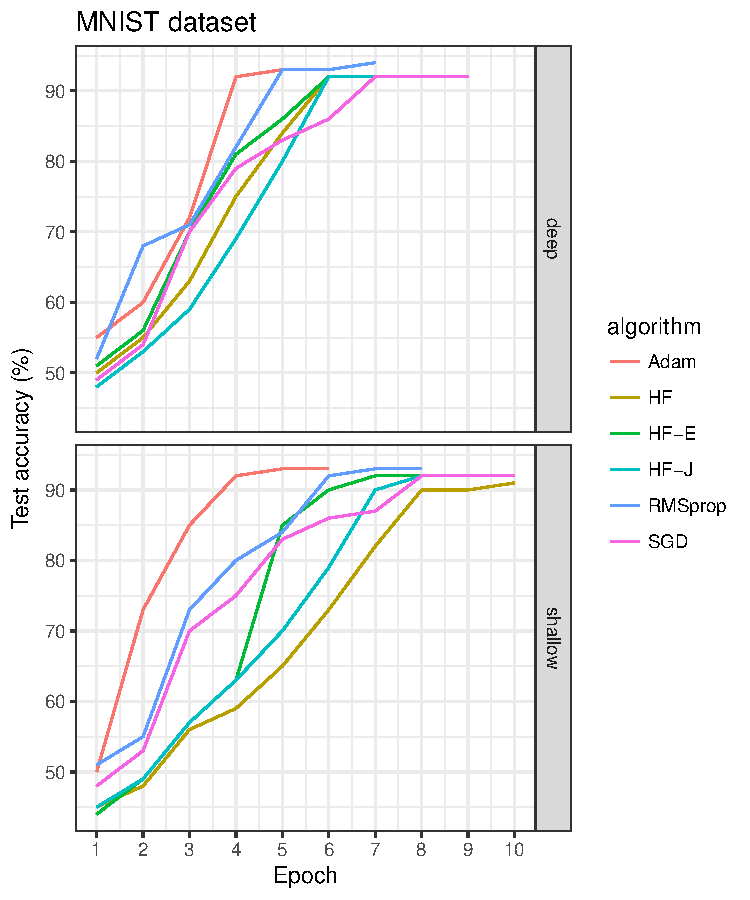
\includegraphics[scale=0.7]{plot_1.pdf}
\caption{Test accuracy (\%) on the MNIST dataset. The upper panel represents deep network architecture while the bottom panel represents shallow network architecture.}
\label{fig:data_mnist_1}
\end{center}
\end{figure}    

In the case of MNIST dataset, most of the optimizers converged to 92 - 93\% accuracy on the test set. Adam converged the fastest of all optimizers. In terms of Hessian free variants of algorithms, there is not a significant difference in their performance and all typically converged to the 93\% accuracy within 8 epochs. However, we notice that in the shallow architecture containing 2 convolutional layers, Hessian free algorithm with no preconditioning took 1 or 2 additional epochs to arrive at the expected accuracy. As for training time-per-epoch on the GPU instance, the architecture with Adam optimizer used on average 5 seconds per epoch, the one with HF-E optimizer used on average 45 seconds per epoch, the one with HF-J optimizer used on average 48 seconds per epoch, and the one with HF optimizer (no preconditioner applied) used on average 75 seconds per epoch. The added computational burden for Hessian free variants compared to first order methods comes from the fact that typically the Hessian free method requires hundreds of CG iterations for one update. In this context, we limit the number of CG iterations to 100. Therefore, making even a single optimization step is fairly computationally expensive relative to first order methods. Adding a preconditioner, either Jacobi or Equilibrium, did help in terms of computational time since it reduced the number of CG iterations. Also, training time with Equilibrium preconditioner was around 60\% less than in case of training Hessian free method with no preconditioner. When comparing the two preconditioners (Equilibrium and Jacobi), we cannot distinguish which one is better with statistical confidence. However, the Equilibrium preconditioner is guaranteed to be at least as robust as (if not better than) the Jacobi preconditioner due to Jansen inequality.
Overall, for all 3 Hessian free methods, training time is comparatively slow (up to two orders of magnitudes slower than in Adam). One of the main reasons is that a relatively large number of Krylov subspace iterations may be required for a solution to approximate the Hessian within each Hessian free iteration. 

\begin{figure}
\begin{center}
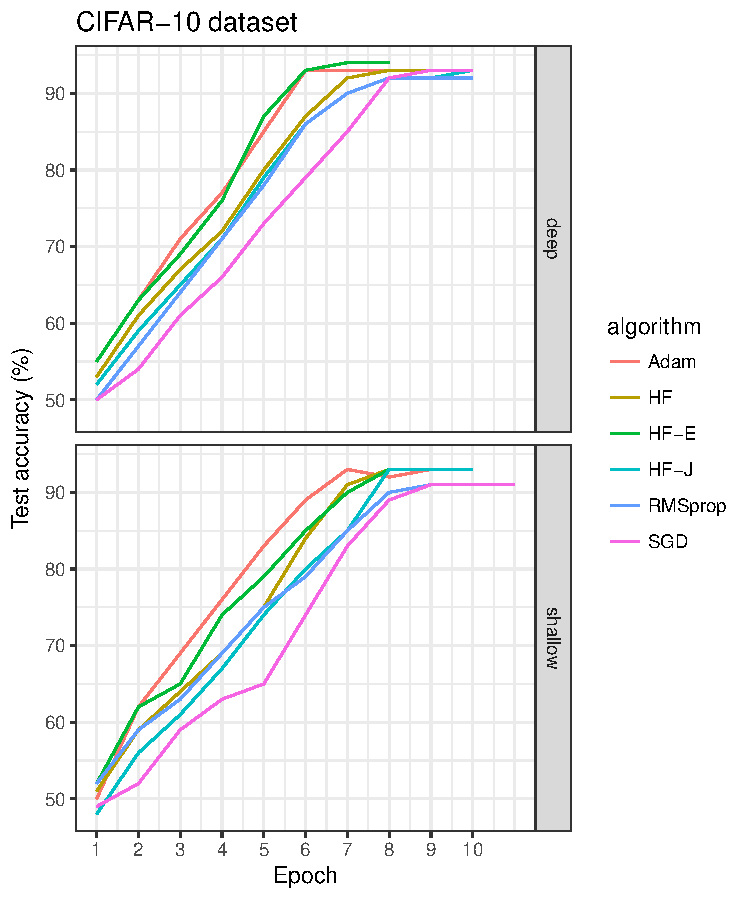
\includegraphics[scale=0.7]{plot_2.pdf}
\caption{Test accuracy (\%) on the CIFAR-10 dataset. The upper panel represents deep network architecture while the bottom panel represents shallow network architecture.}
\label{fig:data_cifar_1}
\end{center}
\end{figure}  

In the CIFAR-10 case, most of the optimizers converged to 92\% - 94\% test accuracy. Both Adam and HF-E converged the fastest; within 6 epochs in the ``deep" convolutional neural network setup, which is encouraging. In terms of training time-per-epoch on the GPU instance, Adam used on average 6 seconds, HF-E used on average 52 seconds, HF-J used on average 55 seconds, and HF (no preconditioning) used on average 83 seconds per epoch. This is slightly longer than in the MNIST case due to 3 RGB channels being used in CIFAR-10.

One generalizable conclusion from both MNIST and CIFAR-10 datasets is that Adam performs slightly better than SGD. Adam offers several advantages over the simple SGD in a sense that Adam uses moving averages of the parameters (momentum). This is beneficial because it enables Adam to use a larger effective step size, helping the algorithm to converge to final step size without fine tuning. A relative downside of Adam is that it requires more computation to be performed for each parameter in each training step in order to maintain the moving averages and variance, and calculate the scaled gradient. Hence, it uses more memory to store the average and variance for each parameter. If this is a problem, a simple SGD could potentially be used instead but more likely it would require more careful hyperparameter tuning (more thorough than what we did with the learning rate) before it could converge as quickly as Adam.

\subsection{The effect of minibatches}  

While Section \ref{sec:prec} discusses results from experiments done on the entire datasets, here we perform the same experiments on mini-batches. An underlying question to consider is how to set the size of the gradient and curvature mini-batches. The answer is typically problem-dependent and specific to the input dimensions and architecture. For instance, inputs with large dimensions (such as 229 $\times$ 229) may require the batch size to be very small if batch normalization is applied. In both datasets, MNIST and CIFAR-10, we set the size of each mini-batch to $2^7$. We use the entire training set  for computing gradients and mini-batches for computing matrix-vector products.
\begin{figure}
\begin{center}
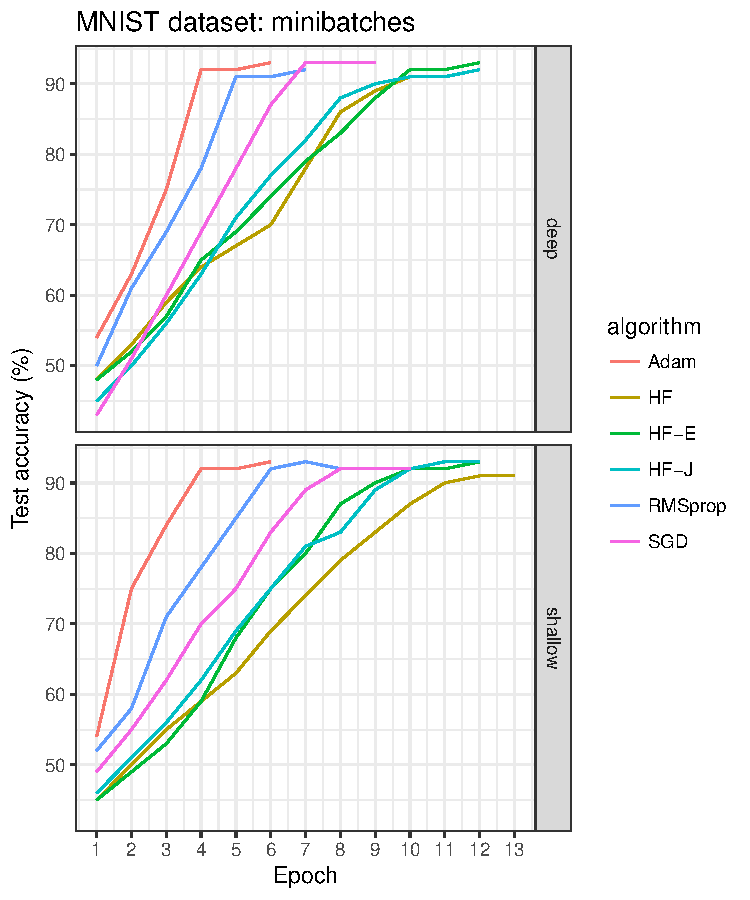
\includegraphics[scale=0.7]{plot_3.pdf}
\caption{Test accuracy (\%) on the MNIST dataset using mini-batches. The upper panel represents deep network architecture while the bottom panel represents shallow network architecture.}
\label{fig:data_mnist_2}
\end{center}
\end{figure}  

\begin{figure}
\begin{center}
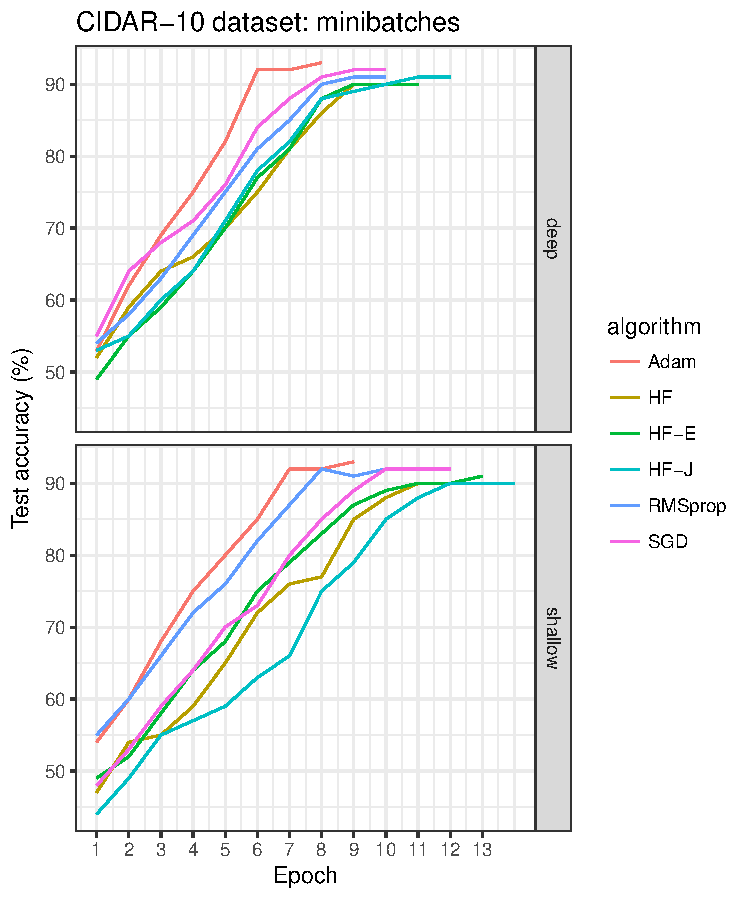
\includegraphics[scale=0.7]{plot_4.pdf}
\caption{Test accuracy (\%) on the CIFAR-10 dataset using mini-batches. The upper panel represents deep network architecture while the bottom panel represents shallow network architecture.}
\label{fig:datacifar_2}
\end{center}
\end{figure}  

In Figure \ref{fig:data_mnist_2}, we compare the test accuracy for different optimizers on the MNIST mini-batch data. We see that Adam performs the best (as expected) but Hessian free variants require more epoch to reach the expected convergence of around 93\% test accuracy. Considering simple models, SGD and Adam will likely find a good fit after one or two passes over the dataset or its mini-batch. It may be difficult for the mini-batch Hessian free method to do much in the same number of gradient and function evaluations. One of the advantages of using mini-batches is a faster training time. For instance, in a mini-batch setting, Adam used on average 5 seconds per epoch, Hessian free with Equilibrium preconditioner used on average 21 seconds per epoch, Hessian free with Jacobi preconditioner used on average 23 seconds per epoch, and Hessian free with no preconditioner used on average 28 seconds per epoch. Hence an important aspect of splitting the dataset into mini-batches is that Hessian-vector multiplications are carried out with a significantly smaller sample size than the one used for the function and gradient. Mini-batches are good for parallelizing computation, especially on GPUs, and lead to faster execution times since computing curvature information on large mini-batches can easily be distributed across several machines.

The similar trend can be seen on experiments from the CIFAR-10 dataset in Figure \ref{fig:datacifar_2}. Adam performs the best and the Hessian-free variants tend to converge more slowly to the expected test accuracy. However, the training time for Hessian free variants in the mini-batch setting was faster: Hessian free with Equilibrium preconditioner used on average 25 seconds per epoch, Hessian free with Jacobi preconditioner used on average 26 seconds per epoch, and Hessian free with no preconditioner used on average 34 seconds per epoch.


\section{Conclusions}

In this paper we explored the performance of different Hessian free methods on the MNIST and CIFAR-10 datasets in the context of convolutional neural network architectures. We also implemented and tested several preconditioners in order to reduce the number of CG iterations. Experiments with these Hessian free variants show better convergence and generalization than RMSprop or SGD method. Moreover, the performance of the Hessian free methods is on par with the Adam optimizer. 

Despite being a promising procedure, the Hessian free method currently faces some formidable challenges amongst machine learning practitioners. One of the main barriers for wide-scale deployment and adoption of the Hessian free methods is their long computational time. The CG routine inside the Hessian free setup requires on the order of $10^2$ to $10^3$ iterations per single step. This means a computational overhead of about $10^2$ to $10^3$ more per iteration, which is a signficant downside to any marginal benefits compared to Adam. To speed up the training and evaluation time for Hessian free methods, one area for potential research may be experimenting with some type of a block-diagonal approximation of the curvature matrix or its sub-sampling in order to improve Hessian free convergence properties. In its essence, the Hessian matrix is closely block-diagonal. Past research on a block-diagonal approximation of the Fisher information matrix showed promising results where training time for a one-layer perceptron was reduced by one order of magnitude ~\cite{LeRoux08}.

However, even after we eliminate the memory concerns, another large downside of a naive application of the Hessian free method is that its gradient and function values must be computed over the entire training set, which could contain hundreds thousands or millions of training examples in the real-world applications. Unlike mini-batch Adam or SGD, getting the Hessian free to work effectively on mini-batches is more tricky. Ideally, the size of the mini-batch should be a hyperparameter itself. It may be worth experimenting with selecting different mini-batches for computing gradient and computing curvature (e.g. gradient mini-batches and curvature mini-batches). Finally, another interesting area for further research is including localized adaptations where the Hessian free routine could adapt its behaviour based on the mini-batch size and number of conjugate gradient iterations (which is not fixed anymore). This behavior is more characteristic of SGD and could be seen as a stochastic variant of the Hessian free method.




   
%-------------------------------------------------------------------------
{\small
\bibliographystyle{ieee}
\bibliography{egbib}}

\end{document}
